% !TEX encoding = UTF-8 Unicode

\documentclass[a4paper]{article}

\usepackage{color}
\usepackage{url}
\usepackage[T2A]{fontenc} 
\usepackage[utf8]{inputenc}
\usepackage{graphicx}

\usepackage[english,serbian]{babel}
\usepackage[unicode]{hyperref}
\hypersetup{colorlinks,citecolor=red,filecolor=green,linkcolor=blue,urlcolor=blue}

\begin{document}

\title{Prednosti tehnologije za prepoznavanje lica\\ \small{Seminarski rad u okviru kursa\\Računarstvo i društvo\\ Matematički fakultet}}

\author{Vuk Stefanović\\ mi19066@alas.matf.bg.ac.rs}
\date{Jun 2023.}
\maketitle

\abstract{
Tema ovog rada je tehnologija za prepoznavanje lica. Rad objašnjava šta predstavlja tehnologija za prepoznavanje lica, njene prednosti, način na koji funkcioniše i gde se primenjuje.
}
\tableofcontents

\newpage

\section{Uvod}
\label{sec:uvod}
Tehnologija za prepoznavanje lica je vrsta biometrijske tehnologije koja koristi algoritme i mašinsko učenje za identifikaciju i verifikaciju identiteta osobe na osnovu njenih crta lica. Poslednjih godina postaje sve popularniji zbog potencijalne primene u različitim industrijama, uključujući bezbednost, marketing i zdravstvenu zaštitu. Softver identifikuje 80 čvornih tačaka na ljudskom licu. U ovom kontekstu, čvorne tačke su krajnje tačke koje se koriste za merenje varijabli lica osobe, kao što su dužina ili širina nosa, dubina očnih duplji i oblik jagodičnih kostiju. Sistem radi tako što hvata podatke za čvorne tačke na digitalnoj slici lica pojedinca i čuva rezultujuće podatke kao otisak lica. Otisak lica se zatim koristi kao osnova za poređenje sa podacima snimljenim sa lica na slici ili video snimku. Iako sistem za prepoznavanje lica koristi samo 80 čvornih tačaka, može brzo i precizno identifikovati ciljne osobe kada su uslovi povoljni.\cite{1}
\begin{figure}[h!]
	\begin{center}
		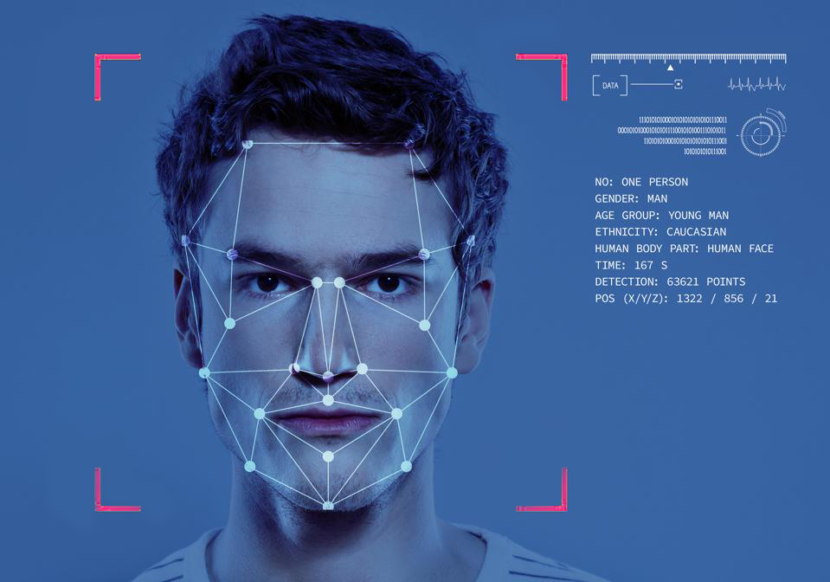
\includegraphics[scale=0.2]{image1.png}
	\end{center}
	\caption{Prikaz na koji način tehnologija za prepoznavanje lica skenira osobu}
\end{figure}


\section{Bezbednost na internetu}
\label{sec:Bezbednost na internetu}
Tehnologija za prepoznavanje lica koristi jedinstvene matematičke obrasce za čuvanje biometrijskih podataka. Stoga je ona među najsigurnijim i najefikasnijim metodama identifikacije u biometrijskoj tehnologiji. Podaci o licu mogu biti anonimizovani i čuvani kao privatni da bi se smanjio rizik od neovlašćenog pristupa. Tehnologija detekcije živosti razlikuje žive korisnike od njihovih slika lica. Ovo sprečava sistem da bude prevaren fotografijom živog korisnika.\cite{2}
Tehnologija prepoznavanja lica može se smatrati bezbednom zbog nekoliko mehanizama i praksi koje su postavljene da zaštite tačnost, privatnost i pouzdanost sistema. Evo kako se postiže sigurnost:
\begin{itemize}
\item Jedinstvene biometrijske osobine -
Lice svake osobe je jedinstveno. Sistemi za prepoznavanje lica koriste specifične karakteristike lica i mere da bi napravili „otisak lica“ koji je teško duplirati
\item  Šifrovanje - Podaci o licu su često šifrovani, što znači da su šifrovani tako da samo ovlašćene strane mogu da ih razumeju. To otežava hakerima pristup i zloupotrebu podataka
\item   Zaštita skladištenja podataka -
Sačuvani podaci o licu čuvaju se u sigurnim bazama podataka, često uz strogu kontrolu pristupa. Ovo sprečava neovlašćeni pristup osetljivim informacijama
\item Kontinuirana poboljšanja -
Programeri uvek rade na poboljšanju algoritama za prepoznavanje lica. Oni koriste velike skupove podataka i napredne tehnike za poboljšanje tačnosti i bezbednosti
\item Višefaktorska autentifikacija -
Za dodatnu sigurnost, prepoznavanje lica se može koristiti zajedno sa drugim metodama, kao što su lozinke ili otisci prstiju. Ovo otežava pristup neovlaš́ćenim korisnicima
\item  Monitoring i revizija -
Organizacije koje koriste prepoznavanje lica često prate i revidiraju svoje sisteme za bilo kakve sumnjive aktivnosti. Ovo pomaže u otkrivanju i sprečavanju kršenja bezbednosti.
\end{itemize}  


\section{Face ID}
\label{sec:faceid}
Face ID (sistem za prepoznavanje lica, koji je dizajnirao i razvio Apple) omogućava korisnicima da otključavaju svoje uređaje, kupuju i pristupaju sigurnim aplikacijama samo jednim pogledom. Koristi poseban sistem kamera, koji se zove„TrueDepth”. ,,TrueDepth” sistem projektuje preko 30.000 nevidljivih tačaka na vaše lice kako bi napravio preciznu mapu vaših karakteristika. Ova mapa se zatim upoređuje sa onom uskladištenom u memoriji vašeg uređaja, da bi se potvrdio vaš identitet. 
Razni telefoni, uključujuć́i najnovije iPhone, koriste Face ID za otključavanje uređaja. Tehnologija nudi zaštitu ličnih podataka i osigurava da osetljivi podaci ostanu nedostupni ako je telefon ukraden. Apple tvrdi da je šansa da slučajno lice otključa vaš telefon otprilike jedan prema milion.\cite{3}
Face ID tehnologija menja igru u svetu bezbednosti i pogodnosti. Korišć́enjem naprednih algoritama za prepoznavanje lica, omoguć́ava korisnicima da otključaju svoje uređaje samo jednim pogledom, čineć́i proces bržim i lakšim nego ikada ranije. Štaviše, Face ID-a takođe pruža visok nivo bezbednosti, uz mere za zaštitu privatnosti i podataka korisnika. A kako tehnologija nastavlja da se razvija, možemo očekivati još uzbudljiviji napredak u narednom periodu.

\begin{figure}[h!]
	\begin{center}
		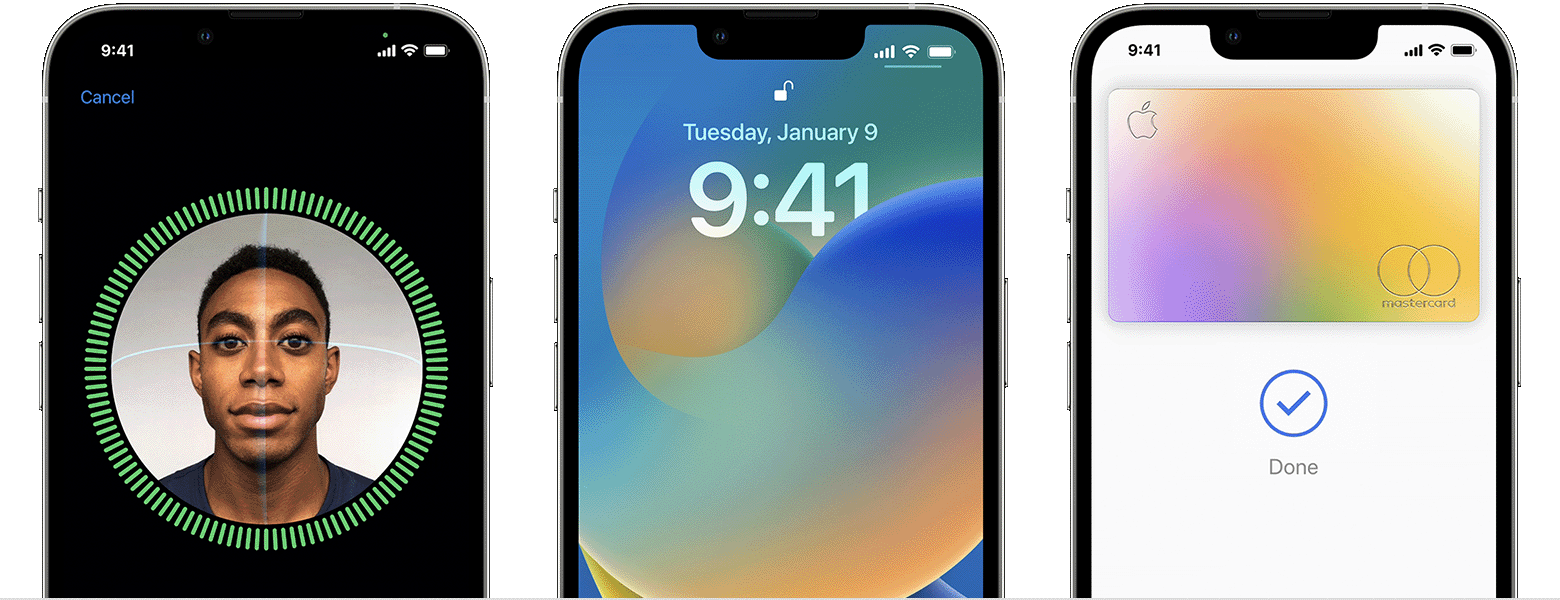
\includegraphics[scale=0.2]{image2.png}
	\end{center}
	\caption{Prikaz kako Face ID funkcionise}
\end{figure}



\section{Ilegalna migracija na granicama}
\label{sec:ilegalne migracije}
Prepoznavanje lica postalo je uobičajen prizor na mnogim aerodromima širom sveta. Veliki broj putnika ima biometrijske pasoše, koji im omogućavaju da preskoče uobičajeno dugačke redove i umesto toga prođu kroz automatizovanu kontrolu e-pasoša kako bi brže stigli do kapije.
Neprecizno posmatranje osobe može biti problematično za zaposlene na carini i graničnoj zaštiti. Zbog toga je granična služba primenila tehnologiju za prepoznavanje lica gde softver, koji je zadužen za kontrolisanje očiju, meri performanse vizuelnog pretraživanja polaznika. Dok upoređuju slike lica Radne stanice prate kretanje očiju preko slika, podučavajući učenike najboljim praksama i veštinama kritičkog vizuelnog prosuđivanja.\cite{ht208108}
Prepoznavanje lica na granici se može takođe koristiti za pronalaženje nestalih osoba i žrtava trgovine ljudima. Pretpostavimo da se nestali pojedinci dodaju u bazu podataka, u tom slučaju, organi za sprovođenje zakona mogu biti upozoreni čim pojedinci budu prepoznati od strane tehnologije za prepoznavanja lica.
Od postavljanja, otprilike u prve tri godine, pre svega u vazduhoplovnom okruženju i donekle u pomorstvu, identifikovali smo oko 300 krijumčara koji koriste ovu tehnologiju. U poslednjih godinu dana na pešačkim kopnenim prelazima na južnoj kopnenoj granici carinici su uhvatili oko 1.000 do 1.100 krijumčara.
\begin{figure}[h!]
	\begin{center}
		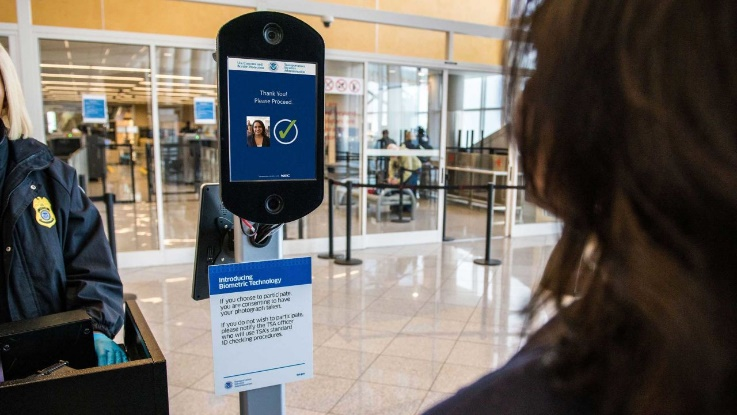
\includegraphics[scale=0.8]{image3.png}
	\end{center}
	\caption{Koršićenje tehnologije za prepoznavanje lica na graničnim prelazima}
\end{figure}

\section{Smanjenje prevara}
\label{sec:smanjenje prevara}
Dokle god postoje mehanizmi verifikacije identiteta, prevaranti će uvek da nađu načine da zaobiđu ove barijere. Među tim tehnikama je lažiranje lica (poznato i kao napadi lažiranja lica), u kojem prevarant pokušava da zaobiđe sistem za prepoznavanje lica i da ga pogrešno identifikuje tako što predstavi lažno lice (npr. fotografiju, 3D modele, 3D štampanu masku). Prevaranti takođe mogu da koriste metode potpomognute veštačkom inteligencijom kao što su ,,deepfakes”, što predstavlja težak izazov za tehnologiju za prepoznavanje lica.\cite{ht20810823} 
Da bi se zaštitili od ovakvih pretnji, evoluirali su sistemi za otkrivanje lažiranja lica, kao što je identifikacija prirodnosti, kako bi se umanjili rizici koji se pojavljuju. Na primer, gledanje teksture lica, gustine crta i odnosa između karakteristika može pomoći da se utvrdi da li je lice stvarno ili ne. Takve tehnologije omoguć́avaju operaterima da dobiju na vremenu, tokom procesa uključivanja, tako što im pomažu u proveravaju pravog identiteta korisnika.
\newpage


\section{Uspesnost brzine pretrage}
\label{sec:brzina pretrage}
Tehnologija prepoznavanja lica je napravila značajan napredak tokom godina i sada može da radi impresivnim brzinama. Brzina tehnologije prepoznavanja lica može da varira na osnovu nekoliko faktora, uključujući hardver koji se koristi, korišćene algoritme i specifičan slučaj upotrebe. Evo nekih opštih smernica:
\begin{itemize}
\item Prepoznavanje u realnom vremenu - Mnogi moderni sistemi za prepoznavanje lica su sposobni za obradu u realnom vremenu, što znači da mogu analizirati i prepoznati lica u deliću sekunde. Ovo je ključno za aplikacije kao što su nadzor, kontrola pristupa i autentifikacija korisnika
\item Okviri u sekundi (FPS) - Brzina prepoznavanja lica se često meri u frejmovima u sekundi  (FPS), što pokazuje koliko pojedinačnih okvira (slika) sistem može da obradi i analizira u jednoj sekundi. Sistemi visokih performansi mogu da postignu stope FPS-a u rasponu od 30 do 60 FPS-a ili čak više
\item   Hardversko ubrzanje - Specijalizovani hardver, kao što su GPU-ovi (Jedinice za grafičku obradu) i TPU-i (Tenzorske procesorske jedinice), može značajno da ubrza zadatke prepoznavanja lica
\item Modeli dubokog učenja - Moderne tehnike prepoznavanja lica često se oslanjaju na modele dubokog učenja, kao što su konvolucione neuronske mreže (CNN), koje su optimizovane za brzinu i tačnost. Ovi modeli mogu efikasno da obrađuju velike količine podataka i da omoguće brže prepoznavanje
\item Ekstrakcija karakteristika - Brzina prepoznavanja lica takođe može zavisiti od toga koliko efikasno sistem izdvaja i obrađuje crte lica. Neki sistemi koriste tehnike za izdvajanje osnovnih crta lica pre pokretanja stvarnog algoritma za prepoznavanje i tako poboljšavaju brzinu obrade
\item Veličina baze podataka - Broj lica u bazi podataka koja se pretražuju takođe utiče na brzinu prepoznavanja. Veće baze podataka zahtevaju više računarskih resursa za uparivanje, što može uticati na ukupne performanse
\item Faktori životne sredine - Kvalitet ulaznih slika, uslovi osvetljenja i složenost pozadine mogu uticati na brzinu i tačnost prepoznavanja lica. Slike lošeg kvaliteta mogu zahtevati više vremena obrade da bi se postigli tačni rezultati
\end{itemize}  

Sve u svemu, tehnologija prepoznavanja lica je napredovala do tačke u kojoj može da izvrši prepoznavanje velike brzine u različitim praktičnim scenarijima. Međutim, važno je napomenuti da stvarna brzina može da varira u zavisnosti od specifične tehnologije koja se koristi i uslova u kojima se primenjuje.\cite{ht208108235}


\section{Zaključak}
\label{sec: zaključak }
Ukratko, tehnologija za prepoznavanja lica značajno je napredovala poslednjih godina i našla je široku primenu u različitim sektorima, postala je bolja zahvaljujući pametnijim algoritmima i bržem hardveru. Odlikuje je preciznost, brzina i to što se primenjuje svuda, od bezbednosti pa sve do zabavnih stvari, ali, takođe izaziva zabrinutost za privatnost i pravičnost. Prepoznavanje lica bi moglo da olakša upotrebu uređaja i da nam pruži više ličnih iskustava – ali moramo da budemo oprezni i da ga pravilno koristimo. Kontinuirano istraživanje, etička razmatranja i čvrsti propisi biće ključni u oblikovanju budućnosti ove tehnologije, dok će istovremeno da osiguraju da ona služi društvu na siguran i pošten način



\addcontentsline{toc}{section}{Literatura}
\appendix

\iffalse
\bibliography{reference} 
\bibliographystyle{plain}
\fi

\begin{thebibliography}{6}

\bibitem{1} \href{https://www.techtarget.com/searchenterpriseai/definition/facial-recognition}{Definition of Facial recognition}
\bibitem{2} \href{https://aws.amazon.com/what-is/facial-recognition/#:~:text=taken%20years%20earlier.-,Is%20facial%20recognition%20safe%3F,identification%20methods%20in%20biometric%20technology}{The benefits of facial recognition technology}
\bibitem{3} \href{https://support.apple.com/en-us/HT208108 }{Face ID advanced technology Apple}
\bibitem{ht208108} \href{https://www.biometricupdate.com/202003/seeing-is-identifying-new-border-protection-systems-train-how-to-spot-impostors }{Border protection systems}
\bibitem{ht20810823} \href{https://www.idnow.io/blog/fraud-detection-anti-spoofing-facial-recognition/ }{Anti-spoofing facial recognition }
\bibitem{ht208108235} \href{https://en.wikipedia.org/wiki/Facial_recognition_system }{Wikipedia Facial recognition system}



\end{thebibliography}

\end{document}
}